\section{General}

I put here a little resume of what's going on at the moment with the examples and the evaluations. This informal text goes on until the \textbf{Data Sets} section. First of all, we differentiate two things: \emph{examples} and \emph{evaluations}. While both are an analysis of several iterations of our model over data sets, examples and evaluations do not run over the same data sets and do not have the same scope. While the evaluations run on the most complex data sets with randomly generated disagreements between the agents, the examples use simple data sets with determined disagreements. The examples test the theoretical foundations of our model by evaluating each disagreement resolution separately in a controlled set of data. On the opposite, the evaluations evaluate the performances of our model over challenging data and unexpected combinations of disagreements.

We work on a total of four data sets: two simple and two complex. The two simple are on the \emph{seat} domain and the \emph{animal} domain, while the two complex are on the \emph{sponge} domain and the \emph{soy bean disease} domain. I will present them better later, but the important numbers are:

\paragraph{Seat:} the instances are created by procedural generation to secure consistency. We initially have three classes on which inductive learners can easily generalize. We can generate as much instances as we want, but I usually work with 50 for each class. This data set is used for the examples of overlap and hypo/hypernymy resolutions that do not have second order disagreements.

\paragraph{Animal:} the instances are animal species dispatched in 7 classes. The description of each specie is an array of bits, each bit coding for the absence or presence of a feature (ex: feather, egg). Only three of the classes have enough instances to be manipulated in order to create custom disagreements. This data set is used for the examples of second order disagreements of interest that we listed.

\paragraph{Sponges:} the instances are sponges of different species (3 classes). Their description is complex and the generalization hard. There is a total of 120 instances in the data set, evenly distributed among the classes. This data set is used to evaluate one overlap or one hypo/hypernymy resolution randomly generated.

\paragraph{Soy Bean Disease:} the instances are ill soy beans classified by probable disease they suffer from (14 classes). While still being complex, the generalization over these classes remains easier than over the sponges. Among the 14 classes, only 6 have enough instances to be manipulated in order to create custom disagreements. This data set is used to evaluate multiple disagreements randomly generated and combined.

By \emph{randomly generated}, I mean that after distributing evenly each instance of each class between the two agents, some of these classes are combined under a same label in order to create a disagreement between the two agents once they learned their initial contrast sets. I will not enter into details now, but an overlap requires three classes (two different pairs of class are combined for each agent), a hypo/hypernymy requires the same pair of classes for each agent (one agent combine it the other don't), a homonymy one different class for each agent (a new label is attributed to both classes) and a synonymy the same class for each agent (a new label is attributed to one of them). Note that an overlap creates two hypo/hypernymy, and a homonymy creates two synonymy.

The method described in the previous paragraph creates first order disagreements when using simple data sets, and frequently second order disagreements when using more complex data sets. In order to create second order disagreements in simple data sets, we have to use a different technique that follows the same logic as for first order disagreements, except that once the initial contrast set is learned we delete some parts of the concept's extensional definition.

Each kind of example / evaluation is tested with both extensive and lazy agents.

The things I evaluate at the moment:

\begin{enumerate}
\item the initial and final precision of the agents
\item the gain of precision after argumentation
\item the number of messages exchanged
\item the number of example exchanged
\item the number of generalization exchanged
\end{enumerate}

I'm planning to add more, after discussion. An important definition: the precision is the number of examples from the overall context (examples from $A_{1}$ $\cup$ examples from $A_{2}$) that are subsumed by one concept for each agent, and for which these two concepts have the same sign.

\subsection{Representing the Containers}

% Introducing the two types of representations for contrast set
A challenge that must be faced when illustrating our experiments, is the representation of the agents' containers in a way that makes apparent the relations between the different concepts. While the pairing relation between two concepts can easily be represented through a Venn diagram, keeping readability on a Venn diagram representing 6 concepts (three being the minimal number of class in the data sets that we use, times two contrast sets) is highly hazardous. Keeping readability on a Venn diagram representing the two time seven classes of the Zoology data set is impossible, not mentioning the two time fourteen classes of the Soybean data set.

% Representing the containers with a table of Venn diagrams
\subsubsection{Table of Venn Diagrams}
The most direct approach to represent the pairing relations between two sets of concepts is the table of Venn diagrams. 

% How we represent the contrast sets
In the present issue, we represent the contrast sets as the schema shown in figure \ref{normalcset}. The bar represents a set of examples. The vertical lines that partition the bar marks the different concepts to which the examples belong, delimiting the extensional definitions. The brackets mark the coverage of the different intensional definitions. By default, these brackets should match the vertical lines of their corresponding extensional definitions. Finally, at the top or the bottom of the bracket, the sign of the concept is indicated. When two contrast sets are represented side-by-side, one of them is represented upside down with regard to the presentation in figure \ref{csetcomparison}. Moreover, a third bar representing the overall context is inserted between the two contrast sets' bars. While this bar does not have signs or intensional definition, it is partitioned accordingly to the categories of the initial data set -- in our case, it represents the seven categories of animal in the zoo data set.

\begin{figure}[t]
\centering
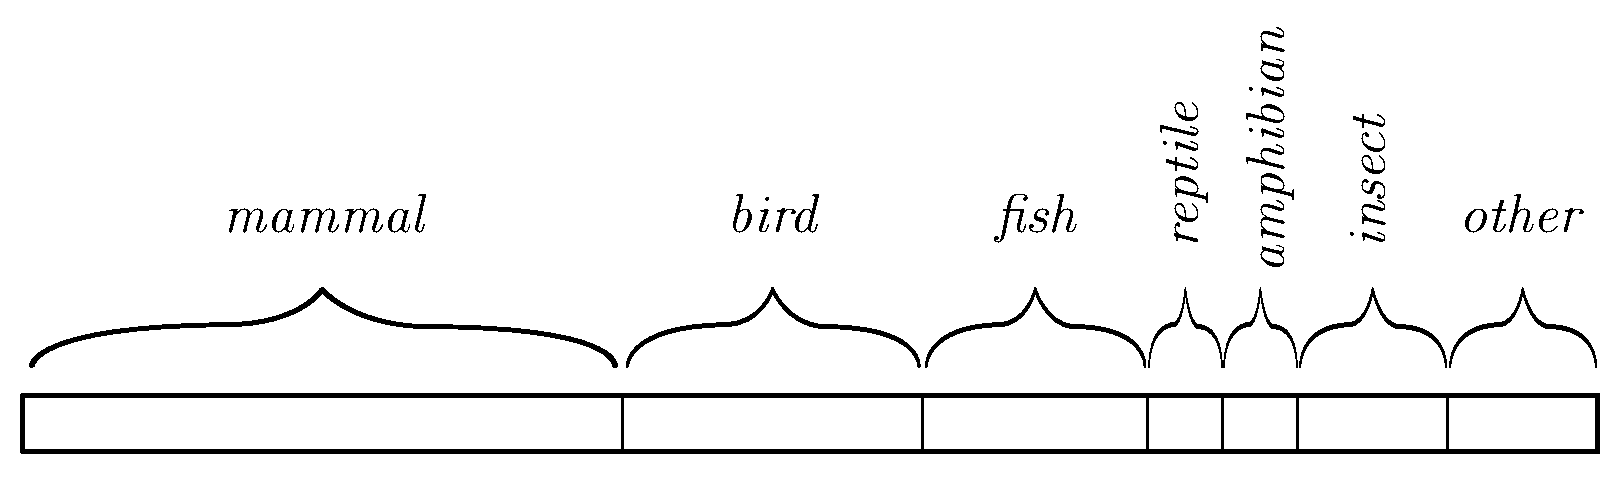
\includegraphics[scale = 0.3]{figs/baceCset.pdf}
\caption{\label{normalcset} Example of contrast set over the zoo data set. The extensional definitions are represented by the partition of the bar, the brackets are symbolizing their respective intensional definitions and their coverage, and finally their signs is written above them.}
\end{figure}

\begin{figure}[t]
\centering
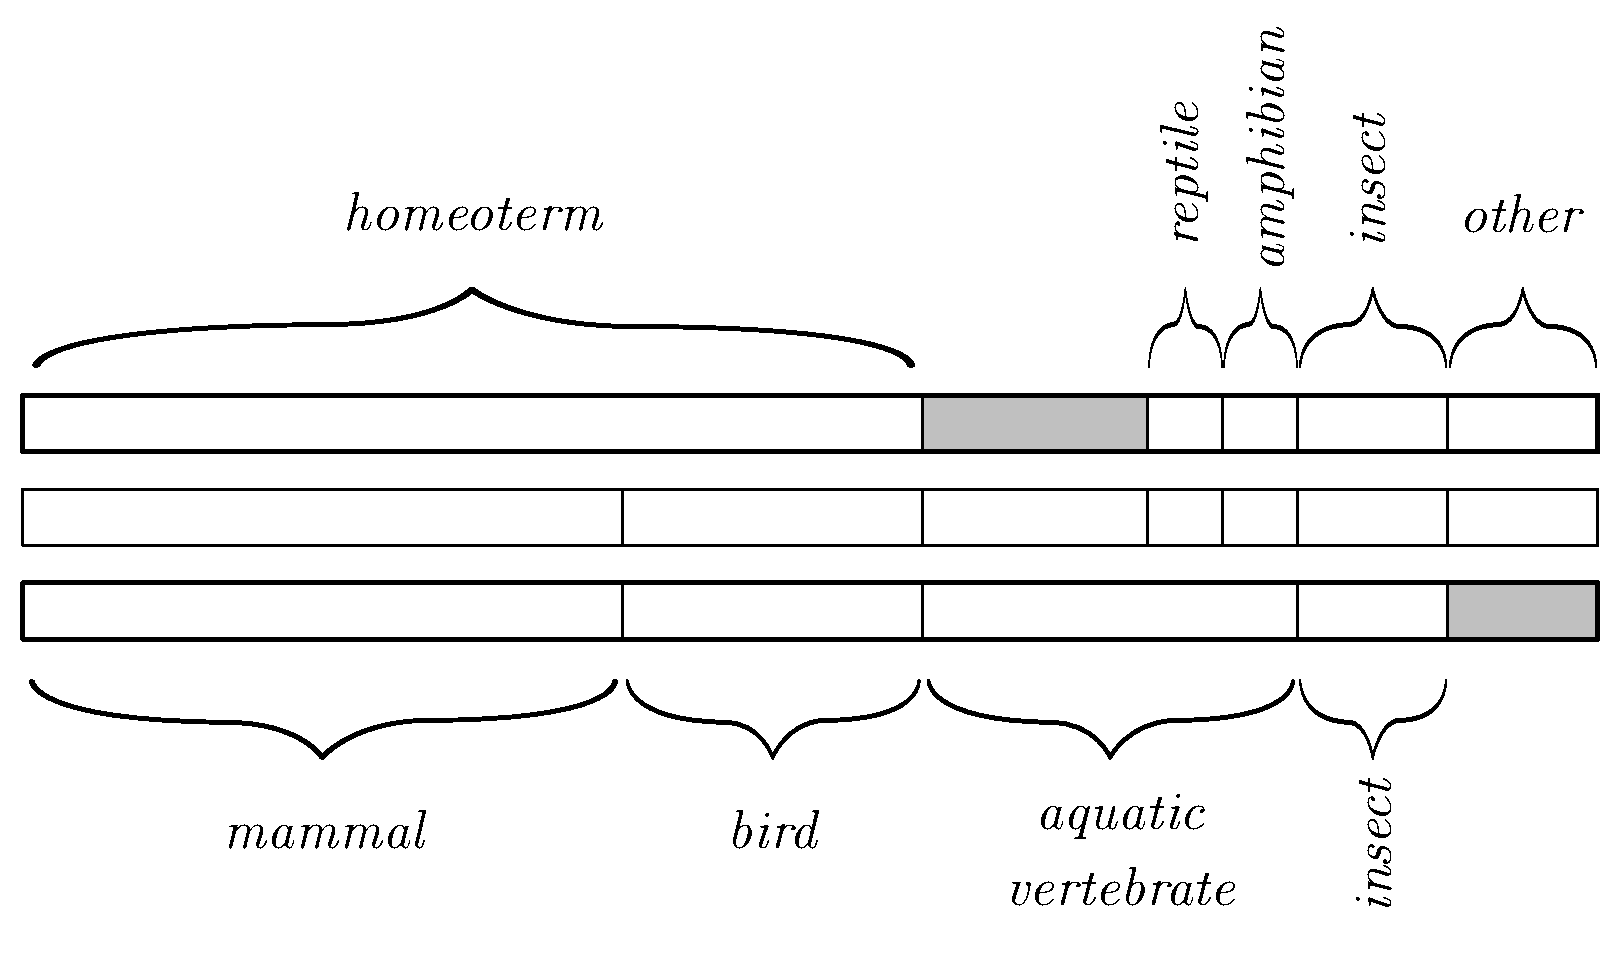
\includegraphics[scale = 0.3]{figs/exampleCsets.pdf}
\caption{\label{csetcomparison} Comparison of two contrast sets. The initial partition of the examples as found in the data set is represented between them. The gray part is representing missing examples from the overall context}.
\end{figure}

\section{Examples of First Order Disagreements}

\subsection{Data and Methodology}

The data set used for experiments on first order disagreements is the \emph{seat} data set, that has been created for the purpose of the present thesis. This data set is automatically generated by a procedural model, and consists of 150 entries divided into 3 categories of 50 instances each: \emph{chair}, \emph{armchair} and \emph{stool}. Each instance has a solution which is the name of a category, and a description. The description is a feature term $X_{i}$ with two main features: \emph{$X_{i}$.back-type} and \emph{$X_{i}$.arm-type}. The instances are generates such that:

\begin{itemize}
\item if the solution is \emph{armchair}, \emph{$X_{i}$.back-type $\doteq$ back} and \emph{$X_{i}$.arm-type $\doteq$ arms}
\item if the solution is \emph{chair}, \emph{$X_{i}$.back-type $\doteq$ back} and \emph{$X_{i}$.arm-type $\doteq$ no-arms}
\item if the solution is \emph{stool}, \emph{$X_{i}$.back-type $\doteq$ no-back} and \emph{$X_{i}$.arm-type $\doteq$ no-arms}
\end{itemize}

The rest of the features are filled with random values. Since they are not linked to the classification of the instances, these additional features should not appear in the generalizations of the agents and are just present as control features.

The data set \emph{seat} is used as a test data set $E_{test}$. Two additional data sets are created in order to be used as learning data sets, one for each agent. The first data set, $E_{t1}$, has 20 generated instances of chair, 20 generated instances of armchair and  10 generated instances of stool. However, the solution of the instances of stool are changed for \emph{chair} without modifying their descriptions. The second data set, $E_{t2}$, has 20 generated instances of chair, 20 generated instances of stool and  10 generated instances of armchair. Again, the solution of the instances of armchair are changed for \emph{chair}. These modifications, illustrated in figure \ref{}, lead to an overlap between the two sets of instances that have now \emph{chair} for solution.

Prior to the argumentation, two semiotic agents $A_{k}$ and $A_{-k}$ learn their initial contrast sets $A_{k}.K_{i}$ and $A_{-k}.K_{i}$ by using \textbf{ABUI} over respectively $E_{t1}$ and $E_{t2}$ as described in section \ref{}. This results in the situation shown in figure \ref{}, where the two concepts $C_{chair}^{k}$ and $C_{chair}^{-k}$ are in a relation of type overlap in the overall context. Since both agents have examples of instances from the three generated categories, this situation does not generate any second order disagreements: $A_{k}$ and $A_{-k}$ will always compute the two same local relations for a given pair of concepts. Once the agents have created their contrast set, they set their state to \emph{Initializing Argumentation}. Then, a token is randomly given to  one of the agent. The agents argue until their list of disagreement has become empty while they are in the \emph{Choosing a Disagreement} state.

\subsection{Exemplifying  Hypo/Hypernymy Disagreement}

In this exemplification, the classes \emph{chair} and \emph{armchair} are merged under the label \emph{chair} in the initial data set dealt to $A_{1}$. Therefore, we have $A_{1}$ that has an initial contrast set containing two concepts \emph{chair} and \emph{stool}, while $A_{2}$ has the standard initial contrast set containing \emph{chair}, \emph{armchair} and \emph{stool}. The initial setup guarantees that the concept \emph{chair} from $A_{2}$ is a hypernym of the concepts \emph{chair} and \emph{armchair} from $A_{2}$: $A_{1}$ learns that a seat is a chair if \emph{$X_{i}$.back-type $\doteq$ back} and a stool if \emph{$X_{i}$.back-type $\doteq$ no-back} and \emph{$X_{i}$.arm-type $\doteq$ no-arms} while $A_{2}$ retrieves correctly the generation rules of \emph{chair}, \emph{armchair} and \emph{stool} presented in the section above. Since the \emph{seat} data set does not pose any problem for inductive learning, the degree of error tolerated by the agents will only be $\tau_{E} = 1$ which is the smallest possible value.

In order to initiate the communication between the agent, the token is dealt to a random agent: let it be $A_{1}$. $A_{1}$ starts in the state 1, and send the intensional definitions $I(Chair^{1})$ and $I(Stool^{1})$ to $A_{2}$. Then $A_{1}$ passes the token to $A_{2}$, which also starts in the state 1, and $A_{2}$ sends the three intensional definitions $I(Armchair^{2})$, $I(Chair^{2})$ and $I(Stool^{2})$ to $A_{1}$. Then $A_{2}$ passes the token to $A_{1}$.

$A_{1}$ receives the token while being in the state 2. $A_{1}$ creates a hypothesis $H_{1}$ with the intensional definitions $I(Armchair^{2})$, $I(Chair^{2})$ and $I(Stool^{2})$ received from $A_{2}$ through the messages \emph{Assert}. Since the examples from the data set seat has been homogeneously distributed among the agents, $A_{1}$ evaluates correctly the relations $Chair^{1} \odot Armchair^{2}$, $Chair^{1} \odot Chair^{2}$ and $Stool^{1} \equiv Stool^{2}$ as its local relations. $A_{1}$ then sends all the r-triplets of its local relations through six messages:

\begin{multicols}{2}
\begin{enumerate}
    \item \emph{evaluation}($Chair^{1}, Armchair^{2}, (1,1,0)$)
    \item \emph{evaluation}($Chair^{1}, Chair^{2}, (1,1,0)$)
    \item \emph{evaluation}($Chair^{1}, Stool^{2}, (1,0,1)$)
    \item \emph{evaluation}($Stool^{1}, Armchair^{2}, (1,0,1)$)
    \item \emph{evaluation}($Stool^{1}, Chair^{2}, (1,0,1)$)
    \item \emph{evaluation}($Stool^{1}, Stool^{2}, (0,1,0)$)
\end{enumerate}
\end{multicols}

Then $A_{1}$ passes the token to $A_{2}$, which is now in state 2 and creates its own hypothesis $H_{2}$ with the intensional definitions $I(Armchair^{1})$ and $I(Chair^{1})$ received from $A_{1}$. As we mentioned in the paragraph above, the homogeneous distribution of the examples allow the agents to find the same relations between the concepts (the local relations are already the same as the overall relations), which means that $A_{2}$ sends the same evaluations to $A_{1}$:

\begin{multicols}{2}
\begin{enumerate}
    \item \emph{evaluation}($Armchair^{2}, Chair^{1}, (0,1,1)$)
    \item \emph{evaluation}($Armchair^{2}, Stool^{1}, (0,1,1)$)
    \item \emph{evaluation}($Chair^{2}, Chair^{1}, (1,0,1)$)
    \item \emph{evaluation}($Chair^{2}, Stool^{1}, (1,0,1)$)
    \item \emph{evaluation}($Stool^{2}, Chair^{1}, (1,0,1)$)
    \item \emph{evaluation}($Stool^{2}, Stool^{1}, (0,1,0)$)
\end{enumerate}
\end{multicols}

When $A_{1}$ receives the token from $A_{2}$, $A_{1}$ is in state 3. $A_{1}$ uses the local r-triplets that it computed in the precedent state along with the r-triplets that it received from $A_{2}$ through the \emph{evaluation} messages, and concludes that the overall relations are the same as its local relations. Therefore, $A_{1}$ does not send any example to $A_{2}$. Finally, $A_{1}$ creates a list $D_{1}$ with the observed disagreements. $A_{1}$ passes the token to $A_{2}$ that accomplishes its turn in state 3, compute the overall relations and draw the same conclusions as $A_{1}$, creates the list $D_{2}$ and passes back the token to $A_{1}$. At this point, after both agents have been thought the third state, the lists of disagreements are:

\begin{itemize}
    \item $D_{1} = [(Chair^{1}, Armchair^{2}, (1,1,0))$, $(Chair^{1}, Chair^{2}, (1,1,0))]$
    \item $D_{2}= [(Armchair^{2}, Chair^{1}, (0,1,1)), (Chair^{2}, Chair^{1}, (0,1,1))]$
\end{itemize}

$A_{1}$ receives the token. Since $A_{1}$ is now in the state 4 and has not received any message \emph{address} from $A_{2}$, $A_{1}$ chooses $Chair^{1}, Armchair^{2}, (1,1,0)$ as a random disagreement from $D_{1}$ and send a message \emph{address}($Chair^{1}, Armchair^{2}$) to $A_{2}$. Since $Chair^{1} \odot Armchair^{2}$, the next state of $A_{1}$ will be the state 5. $A_{1}$ passes the token to $A_{2}$, and $A_{2}$ receives the message \emph{address}($Chair^{1}, Armchair^{2}$). Since $Armchair^{2} \odot Chair^{1}$, the next state of $A_{2}$ will be the state 5.

At the beginning of its turn, $A_{1}$ creates the extensional definition of the concept $new_1$ that $A_{1}$ and $A_{2}$ will create to resolve the disagreement $Chair^{1}, Armchair^{2}, (1,1,0)$. This new concept will be the co-hyponym of $Chair^{1}$ with $Armchair^{2}$. Consequently, $A_{1}$ builds the set of positive examples $E^{1}_{+} = E(Chair^{1}) - E(Armchair^{2'})$ and the set of negative examples $E^{1}_{-} = E_{K1} - E^{1}_{+}$. Then, $A_{1}$ passes the token to $A_{2}$ which creates the sets $E^{2}_{+} = E(Chair^{1'}) - E(Armchair^{2})$ and $E^{2}_{-} = E_{K2} - E^{2}_{+}$. Due to the experimental setup of this example, each set $E^{x}_{+}$ will contain the examples with the features \emph{$X_{i}$.back-type $\doteq$ back} and \emph{$X_{i}$.arm-type $\doteq$ no-arms} of the context $E_{Kx}$.

The agents $A_{1}$ and $A_{2}$ will now enter in a loop from which they will exit only once they have each found an intensional definition, $I^{1}_{+}$ and $I^{2}_{2}$, that can be the intensional definition of  \emph{both} $E^{1}_{+}$ and $E^{2}_{+}$. When $A_{1}$ starts in state 6, it creates an intensional definition $I^{1}_{+}$ and sends it to $A_{2}$ with a message \emph{Assert}($new_1$, $I^{1}_{+}$). After receiving the token, $A_{2}$ creates its intensional definition  $I^{2}_{+}$ and sends a message \emph{Assert}($new_1$, $I^{2}_{+}$) to $A_{1}$. Additionally, $A_{2}$ evaluates the intensional definition $I^{1}_{+}$ that it received. Since $I^{1}_{+}$ subsumes all the examples from $E^{2}_{+}$ without subsuming any examples from $E^{2}_{-}$, $A_{2}$ also send a message \emph{accept}($new_1$, $I^{1}_{+}$) to $A_{1}$. When $A_{1}$ receives the token, $A_{1}$ acknowledges that $A_{2}$ agreed upon the intensional definition $I^{1}_{+}$ through a message \emph{agree}. Then, $A_{1}$ evaluates the intensional definition $I^{2}_{+}$ that it received and notices that $I^{2}_{+}$ subsumes all the examples from $E^{1}_{+}$ without subsuming any example from $E^{1}_{-}$. Therefore, $A_{1}$ sends a message \emph{agree}($new_1, I^{2}_{+}$) to $A_{2}$. Now that $A_{1}$ has agreed upon the intensional definition of $A_{2}$ and knows that $A_{2}$ agreed upon its intensional definition, $A_{1}$ is ready to move to the state 7. When $A_{2}$ gets the token, it is notified by $A_{1}$ that $I^{2}_{+}$ has been agreen upon. $A_{2}$ is now also ready to move to the state 7.

At the end of the state 6, both agents have found in parallel a similar intensional definition:

\begin{itemize}
    \item $I^{1}_{+}$ = \emph{$X_{i}$.back-type $\doteq$ back} and \emph{$X_{i}$.arm-type $\doteq$ no-arms}
    \item $I^{2}_{+}$ = \emph{$X_{i}$.back-type $\doteq$ back} and \emph{$X_{i}$.arm-type $\doteq$ no-arms}
\end{itemize}

$A_{1}$ is now in state 7 and creates a new concept $new_1^{1}$. Since the current disagreement ($Chair^{1}$, $Armchair^{2}$, $(1,1,0)$) is a hypo/hypernymy disagreement, and since $Armchair^{2}$ belongs to $A_{2}$'s contrast set, $A_{1}$ also create a concept $new_2^{1}$ and remove $Armchair^{2'}$ from $H_{1}$. When $A_{2}$ gets the token, it creates the concept $new_1^{2}$. Since $Armchair^{2}$ belongs to $K_{2}$, $A_{2}$ removes $Armchair^{2}$ from $K_{2}$ and creates a new concept $new_2^{2}$. The composition of the new concepts are the following:

\begin{itemize}
    \item $new_1^{1} = (new_1, I^{1}_{+}, E^{1}_{+})$
    \item $new_2^{1} = (new_2, I(Armchair^{2}), E(Armchair^{2'}))$
    \item $new_1^{2} = (new_1, I^{2}_{+}, E^{2}_{+})$
    \item $new_2^{2} = (new_2, I(Armchair^{2}), E(Armchair^{2}))$
\end{itemize}

Since the current disagreement is a hypo/hypernymy disagreement, the next state of $A_{1}$ and $A_{2}$ is the state 8. $A_{1}$ deletes the hypernym $Chair^{1}$ from $K_{1}$, then passes the token to $A_{2}$ that deletes $Chair^{1'}$ from $H_{2}$. Moving to the state 9, $A_{1}$ evaluates the relations between $new_1^{1}$, $new_2{1}$ and the concepts from $K_{2}$ and sends them to $A_{2}$ through \emph{evaluation} messages:

\begin{multicols}{2}
\begin{enumerate}
    \item \emph{evaluation}($new_1^{1}, Chair^{2}, (0,1,0)$)
    \item \emph{evaluation}($new_1^{1}, Stool^{2}, (1,0,1)$)
    \item \emph{evaluation}($new_2^{1}, Chair^{2}, (1,0,1)$)
    \item \emph{evaluation}($new_2^{1}, Stool^{2}, (1,0,1)$)
\end{enumerate}
\end{multicols}

Then $A_{1}$ passes the token to $A_{2}$ which does the same and sends to $A_{1}$:

\begin{multicols}{2}
\begin{enumerate}
    \item \emph{evaluation}($new_1^{2}, Stool^{1}, (1,0,1)$)
    \item \emph{evaluation}($new_2^{2}, Stool^{1}, (1,0,1)$)
\end{enumerate}
\end{multicols}

$A_{1}$ receives the token and goes through the state 10, where $A_{1}$ computes the overall relations between the new concepts and the old ones by adding $new_1^{1}$ and $new_2^{1}$ to both $K_{1}$ and $H_{1}$. Then, $A_{1}$ observes that $new_1^{1} \equiv Chair^{2}$ and deletes $Chair^{2}$ from $H_{1}$. $A_{1}$ finishes its turn by updating the list of disagreement $D_{1}$, that becomes empty.

When $A_{2}$ receives the token, it computes the overall relations and add $new_1^{2}$ and $new_2^{2}$ to both $K_{2}$ and $H_{2}$. Since $new_1^{1} \equiv Chair^{2}$, $A_{2}$ deletes $Chair^{2}$ from $K_{2}$. $A_{2}$ finishes its turn by updating the list of disagreement $D_{2}$, that also becomes empty.

Going back to state 4, $A_{1}$ finds $D_{1}$ empty, which means that its next state will be the state 12. When $A_{2}$ receives the token, it finds $D_{2}$ empty: its next state will also be 12.



\section{Examples of Second Order Disagreements}

The following section will present four examples of argumentation in the situation where semiotic agents have to face second order disagreements, corresponding to the four cases of second order disagreement highlighted in the figure \ref{}. The examples will use the data set \emph{zoology}, which is more diverse than \emph{seat} with seven classes. However, the ontological structure of \emph{zoology} is more simple than \emph{seat} with a depth of one, making it similar to description logic as the examples are represented as vectors of features' values.

This data set is perfect to test the argumentation involving second order disagreements. On the contrary to the section \ref{} where each agent had distinct contexts, the experiments on second order disagreements involve two agents sharing almost all of the examples from their context. The only examples that are present in only one context are selected to cause the second order disagreements, enabling one agent to see a relation between to concepts with more accuracy than an other. 

\subsection{Data and Methodology}

% Presentation of the Zoology Data Set
The data set used for experiments on second order disagreements is the \emph{zoology} data set from the UCI Machine Learning Repository\footnote{http://archive.ics.uci.edu/ml/datasets/zoo}.
%% Presentation of the different categories
The data set contains animal species as instances, clustered into seven distinct categories. The label of these categories will be listed, followed by their corresponding number of instances between parentheses: \emph{mammal}(41), \emph{bird}(20), \emph{reptile}(5), \emph{fish}(13), \emph{amphibian}(4), \emph{insect}(8) and \emph{other}(10). There is a total of 101 instances in the data set. During the rest of the section, regarding the notation $C_{i}^{k}$, the following abbreviations will be used instead of the full sign \emph{i}: \emph{mammal} = \emph{mam}, \emph{reptile} = \emph{rep}, \emph{amphibian} = \emph{amph} and \emph{insect} = \emph{ins}.
%% Presentation of the different attributes (features)
Each instance has a \emph{sort} (see $\psi$-term formalism) with two main features: a solution (the label of the instance's category) and a description. The description is an array of 17 attributes that can have either a boolean or a numeric value: for instance, the number of legs of the specie or 0 and 1 if the feature is boolean, such as \emph{lactation}.

\subsubsection{Setting Up Contrast Sets for the Examples}

% Creating the contrast sets
Contrast sets learned over the same data sets are remarkably consistent: two contrast sets created over the same data set are usually in synchronic agreement even with a value of $t = 1$. This is at least the case for simple contrast sets like \emph{seat} and \emph{zoology}. In order to prove this, we have evaluated the measures $m_{1}$, $m_{2}$ and $m_{3}$ over 100 creations of contrast sets $A_{k}.K$ and $A_{-k}.K$ using \emph{zoology}. In all the hundred of trials, $A_{k}.K$ and $A_{-k}.K$ were always satisfying contrast sets without any synchronic disagreements ($m_{1}$, $m_{2}$ and $m_{3}$ = 0). Measuring $m_{4}$ to evaluate the diachronic agreement was meaningless since no argumentation held place, thus $A_{k}.K = A_{k}.K_{i}$. Consequently to the absence of disagreement between two agents having this version of the contrast set, any arising disagreement in our scenario can only be caused by the experimental setup that we will introduce.

There are two possible modifications of the contrast sets that can provoke a situation of synchronic disagreement. The first modification consists in changing the label of some instances in the data set, as instances of stools and armchairs have been relabeled as \emph{chair} in the section \ref{}. However, it is impossible to create second order disagreements with such modifications as it does not alter the examples of the contrast sets' context. The only way to create second order disagreement is by deleting some instances from the data set, in order to introduce differences between the contrast sets' context.

\subsubsection{Setting Up the First Case of Second Order Disagreement}

The first case of second order disagreement is due to an overall relation of type overlap. In order to create this overlap, we changing the labels \emph{mammal} and \emph{fish} to $s_{1}$ in $E_{l1}$ and the labels of \emph{fish} and \emph{bird} to $s_{2}$ in $E_{l2}$. This way, the relation $ov.r(C_{1}^{1}, C_{2}^{2})$ is of type overlap. At this point, the local relations $r(C_{1}^{1},C_{2}^{1},A_{1}.E_{K})$ and $r(C_{2}^{2},C_{1}^{2},A_{2}.E_{K})$ will also be of type overlap since they can partition the overall context.

In the first case of second order disagreement, $A_{1}$'s local relation is of type equivalence, which means that $E_{1}^{1}$ and $E_{2}^{1}$ should contain the same examples. For this reason, once the contrast set has been learned, we delete the examples of $E_{mam}$ and $E_{bird}$ from $A_{1}.E_{K}$, leaving only the examples of $E_{fish}$ to be subsumed by both $I_{1}^{1}$ and $I_{2}^{1}$. $A_{1}$ now sees its local relation $r(C_{1}^{1},C_{2}^{1},A_{1}.E_{K})$ as of the equivalence type. Since $I_{mam}^{1}$ is not covering any example anymore, $C_{mam}^{1}$ is deleted from $A_{1}.K$.

In the first case of second order disagreement, $A_{2}$'s local relation is of disjunction type, which means that $E_{1}^{2}$ and $E_{2}^{2}$ should not have any example in common. For this reason, once the contrast set has been learning, we delete the examples of $E_{fish}$ from $A_{2}.E_{K}$, leaving no example to be subsumed by both $I_{1}^{2}$ and $I_{2}^{2}$. $A_{2}$ now sees its local relation $r(C_{2}^{2},C_{1}^{2},A_{2}.E_{K})$ as of the disjunction type.

\subsubsection{Setting Up the Second Case of Second Order Disagreement}

This is similar to first case of second order disagreement, but EXPLAIN HERE DIFFERENCE the second case of second order disagreement is due to an overall relation of type overlap. In order to create this overlap, we proceed as in section \ref{} by changing the labels \emph{mammal} and \emph{fish} to $s_{1}$ in $E_{l1}$ and the labels of \emph{fish} and \emph{bird} to $s_{2}$ in $E_{l2}$. The relation $ov.r(C_{1}^{1}, C_{2}^{2})$ and the local relations $r(C_{1}^{1},C_{2}^{1},A_{1}.E_{K})$ and $r(C_{2}^{2},C_{1}^{2},A_{2}.E_{K})$ are of type overlap again.

In the second case of second order disagreement, $A_{1}'s$ local relation is of type inclusion. One of the sets $E_{1}^{1}$ and $E_{2}^{1}$ should be a subset of the other. For this reason, once the contrast set has been learned, we delete the examples of $E_{mam}$ from $A_{1}.E_{K}$, leaving only the examples of $E_{fish}$ to be subsumed by $I_{1}^{1}$ but both the examples of $E_{fish}$ and $E_{bird}$ to be subsumed by $I_{2}^{1}$. $A_{1}$ now sees its local relation $r(C_{1}^{1},C_{2}^{1},A_{1}.E_{K})$ as of the inclusion type, with $h(C_{1}^{1},C_{2}^{1}, \subset)$.

Similarly to the first case of second order disagreement, in the second case of second order disagreement $A_{2}$'s local relation is of type disjunction. For this reason, we proceed as in the first case of second order disagreement and once the contrast set has been learning, we delete the examples of $E_{fish}$ from $A_{2}.E_{K}$, leaving no example to be subsumed by both $I_{1}^{2}$ and $I_{2}^{2}$. $A_{2}$ now sees its local relation $r(C_{2}^{2},C_{1}^{2},A_{2}.E_{K})$ as of the disjunction type.
 
\subsubsection{Setting Up the Third Case of Second Order Disagreement}

The third case of second order disagreement is due to an overall relation of type inclusion. In order to create this inclusion, we change the label \emph{mammal} to $s_{1}$ in $E_{L1}$ and the labels  \emph{mammal} and \emph{fish} to $s_{2}$ in $E_{l2}$. The relation $ov.r(C_{1}^{1}, C_{2}^{2})$ and the local relations $r(C_{1}^{1},C_{2}^{1},A_{1}.E_{K})$ and $A_{2}$ are of type inclusion, with $h(C_{1}^{1},C_{2}^{1}, \subset)$.

In the third case of second order disagreement, $A_{1}'s$ local relation is of type equivalence, which means that $E_{1}^{1}$ and $E_{2}^{1}$ should contain the same examples. For this reason, once the contrast set has been learned, we delete the examples from  $E_{fish}$ from $A_{1}.K$. This leaves only the examples from $E_{mam}$ to be subsumed by both $I_{1}^{1}$ and $I_{2}^{1}$. $A_{1}$ now sees its local relation $r(C_{1}^{1},C_{2}^{1},A_{1}.E_{K})$ as of the equivalence type. Since $I_{fish}^{1}$ is not covering any example anymore, $C_{fish}^{1}$ is deleted from $A_{1}.K$.

There is no need to change anything from $A_{2}$'s contrast set, since $A_{2}$ already sees its local relation $r(C_{2}^{2},C_{1}^{2},A_{2}.E_{K})$ as of the inclusion type.

\subsubsection{Setting Up the Fourth Case of Second Order Disagreement}

The fourth case of second order disagreement is due to an overall relation of type overlap but is better described as consisting of 
 three sub-cases $c_{1}$, $c_{2}$ and $c_{3}$. In order to create this overlap, we proceed as for setting up the first and second cases of second order disagreement: by changing the labels \emph{mammal} and \emph{fish} to $s_{1}$ in $E_{l1}$ and the labels of \emph{fish} and \emph{bird} to $s_{2}$ in $E_{l2}$. The relation $ov.r(C_{1}^{1}, C_{2}^{2})$ and the local relations $r(C_{1}^{1},C_{2}^{1},A_{1}.E_{K})$ and $r(C_{2}^{2},C_{1}^{2},A_{2}.E_{K})$ are of type overlap.

The particularity of all the cases regrouped as the fourth case of second order disagreement is that $A_{2}$'s local relation $r(C_{2}^{2},C_{1}^{2},A_{2}.E_{K})$ is of type overlap, which means that we do not change anything to $A_{2}$'s contrast set.

However, the local relations of $A_{1}$ in $c_{1}$, $c_{2}$ and $c_{3}$ are respectively of type equivalence, inclusion and disjunction (see figure \ref{fig:VennCases}). For this reason, in $c_{1}$ we will modify the contrast set $A_{1}.K$ as in the set up of the first case of second order disagreement. We delete the examples of $E_{mam}$ and $E_{bird}$ from $A_{1}.E_{K}$ such that $A_{1}$ now sees its local relation $r(C_{1}^{1},C_{2}^{1},A_{1}.E_{K})$ as of the equivalence type.

In $c_{3}$, $A_{1}.K$ is modified as in the set up of the second case of second order disagreement by deleting the examples of $E_{mam}$ from $A_{1}.E_{K}$ such that $A_{1}$ now sees its local relation $r(C_{1}^{1},C_{2}^{1},A_{1}.E_{K})$ as of the disjunction type.

Finally, in $c_{2}$, the examples from $E_{mam}$ are removed from $A_{1}.E_{K}$, leaving only the examples of $E_{fish}$ to be subsumed by $I_{1}^{1}$ but both the examples of $E_{fish}$ and $E_{bird}$ to be subsumed by $I_{2}^{1}$. This causes $A_{1}$ to see its local relation $r(C_{1}^{1},C_{2}^{1},A_{1}.E_{K})$ as of the inclusion type, with $h(C_{1}^{1},C_{2}^{1}, \subset)$.

\section{Evaluation of the Systematic Approach}

\section{Evaluation of the Lazy Approach}